%%%%%%%%%%%%%%%%%%%%%%%%%%%%%%%%%%%%%%%%%
% Structured General Purpose Assignment
% LaTeX Template
%
% This template has been downloaded from:
% http://www.latextemplates.com
%
% Original author:
% Ted Pavlic (http://www.tedpavlic.com)
% Edits by Kevin McClure
%
% Note:
% The \lipsum[#] commands throughout this template generate dummy text
% to fill the template out. These commands should all be removed when 
% writing assignment content.
%
%%%%%%%%%%%%%%%%%%%%%%%%%%%%%%%%%%%%%%%%%

%----------------------------------------------------------------------------------------
%	PACKAGES AND OTHER DOCUMENT CONFIGURATIONS
%----------------------------------------------------------------------------------------

\documentclass{article}

\usepackage{fancyhdr} % Required for custom headers
\usepackage{lastpage} % Required to determine the last page for the footer
\usepackage{extramarks} % Required for headers and 
\usepackage{enumerate}
\usepackage{graphicx} % Required to insert images
\usepackage{lipsum} % Used for inserting dummy 'Lorem ipsum' text into the template
\usepackage{amsmath}
\usepackage{hyperref}

% Margins
\topmargin=-0.45in
\evensidemargin=0in
\oddsidemargin=0in
\textwidth=6.5in
\textheight=9.0in
\headsep=0.25in 

\linespread{1.1} % Line spacing

% Set up the header and footer
\pagestyle{fancy}
\lhead{\hmwkAuthorName} % Top left header
\chead{\hmwkClass : \hmwkTitle} % Top center header
\rhead{\firstxmark} % Top right header
\lfoot{\lastxmark} % Bottom left footer
\cfoot{} % Bottom center footer
\rfoot{Page\ \thepage\ of\ \pageref{LastPage}} % Bottom right footer
\renewcommand\headrulewidth{0.4pt} % Size of the header rule
\renewcommand\footrulewidth{0.4pt} % Size of the footer rule

\setlength\parindent{0pt} % Removes all indentation from paragraphs

   
%----------------------------------------------------------------------------------------
%	NAME AND CLASS SECTION
%----------------------------------------------------------------------------------------

\newcommand{\hmwkTitle}{Lab 1} % Assignment title
\newcommand{\hmwkDueDate}{Monday, September 23, 2013} % Due date
\newcommand{\hmwkClass}{Principles of Engineering} % Course/class
\newcommand{\hmwkAuthorName}{Justin Poh and Sophia Seitz} % Your name

%----------------------------------------------------------------------------------------
%	TITLE PAGE
%----------------------------------------------------------------------------------------

\title{
\vspace{2in}
\textmd{\textbf{\hmwkClass:\ \hmwkTitle}}\\
\normalsize\vspace{0.1in}\small{Due\ on\ \hmwkDueDate}\\
\vspace{3in}
}

\author{\textbf{\hmwkAuthorName}}
\date{} % Insert date here if you want it to appear below your name

%----------------------------------------------------------------------------------------

\begin{document}

\maketitle
\newpage
\section{Introduction} \ \\
For this lab, our task was to design and build a LIDAR out of two servos, an arduino, and an infrared range finder. \\

In order to achieve this, we split the project into two main components. Firstly, we needed a mechanical design that would support sensor such that it was capable of panning (left-right movement) and tilting (up-down movement). This would allow our sensor to scan any point in 3D space within the 180 degree viewing angle it had in front of it. \\

For our software, we decided to give python ultimate control over the process because we wanted a one-button-push implementation such that once the python programme was run, the programme would control the arduino to do what it needed to do and simply produce the plot on screen at the end of the programme.

\section{Mechanical Design}\ \\
Since we decided to focus less on the mechanical design aspect and more on the software aspect, there will not be too much detail presented here on the mechanical design. \\

Essentially we knew we needed a pan and tilt head that would ensure that the sensor panned and tilted while remaining centred along the the axes of rotation. Hence, we chose a cantilever design consisting of the panning servo mounted inside a box. An L-bracket cantilever was used to support the tilt servo and the sensor was mounted to a piece of wood that was glued to the tilt servo to achieve tilting ability. \\
%
\begin{figure}[h!]
\begin{center}
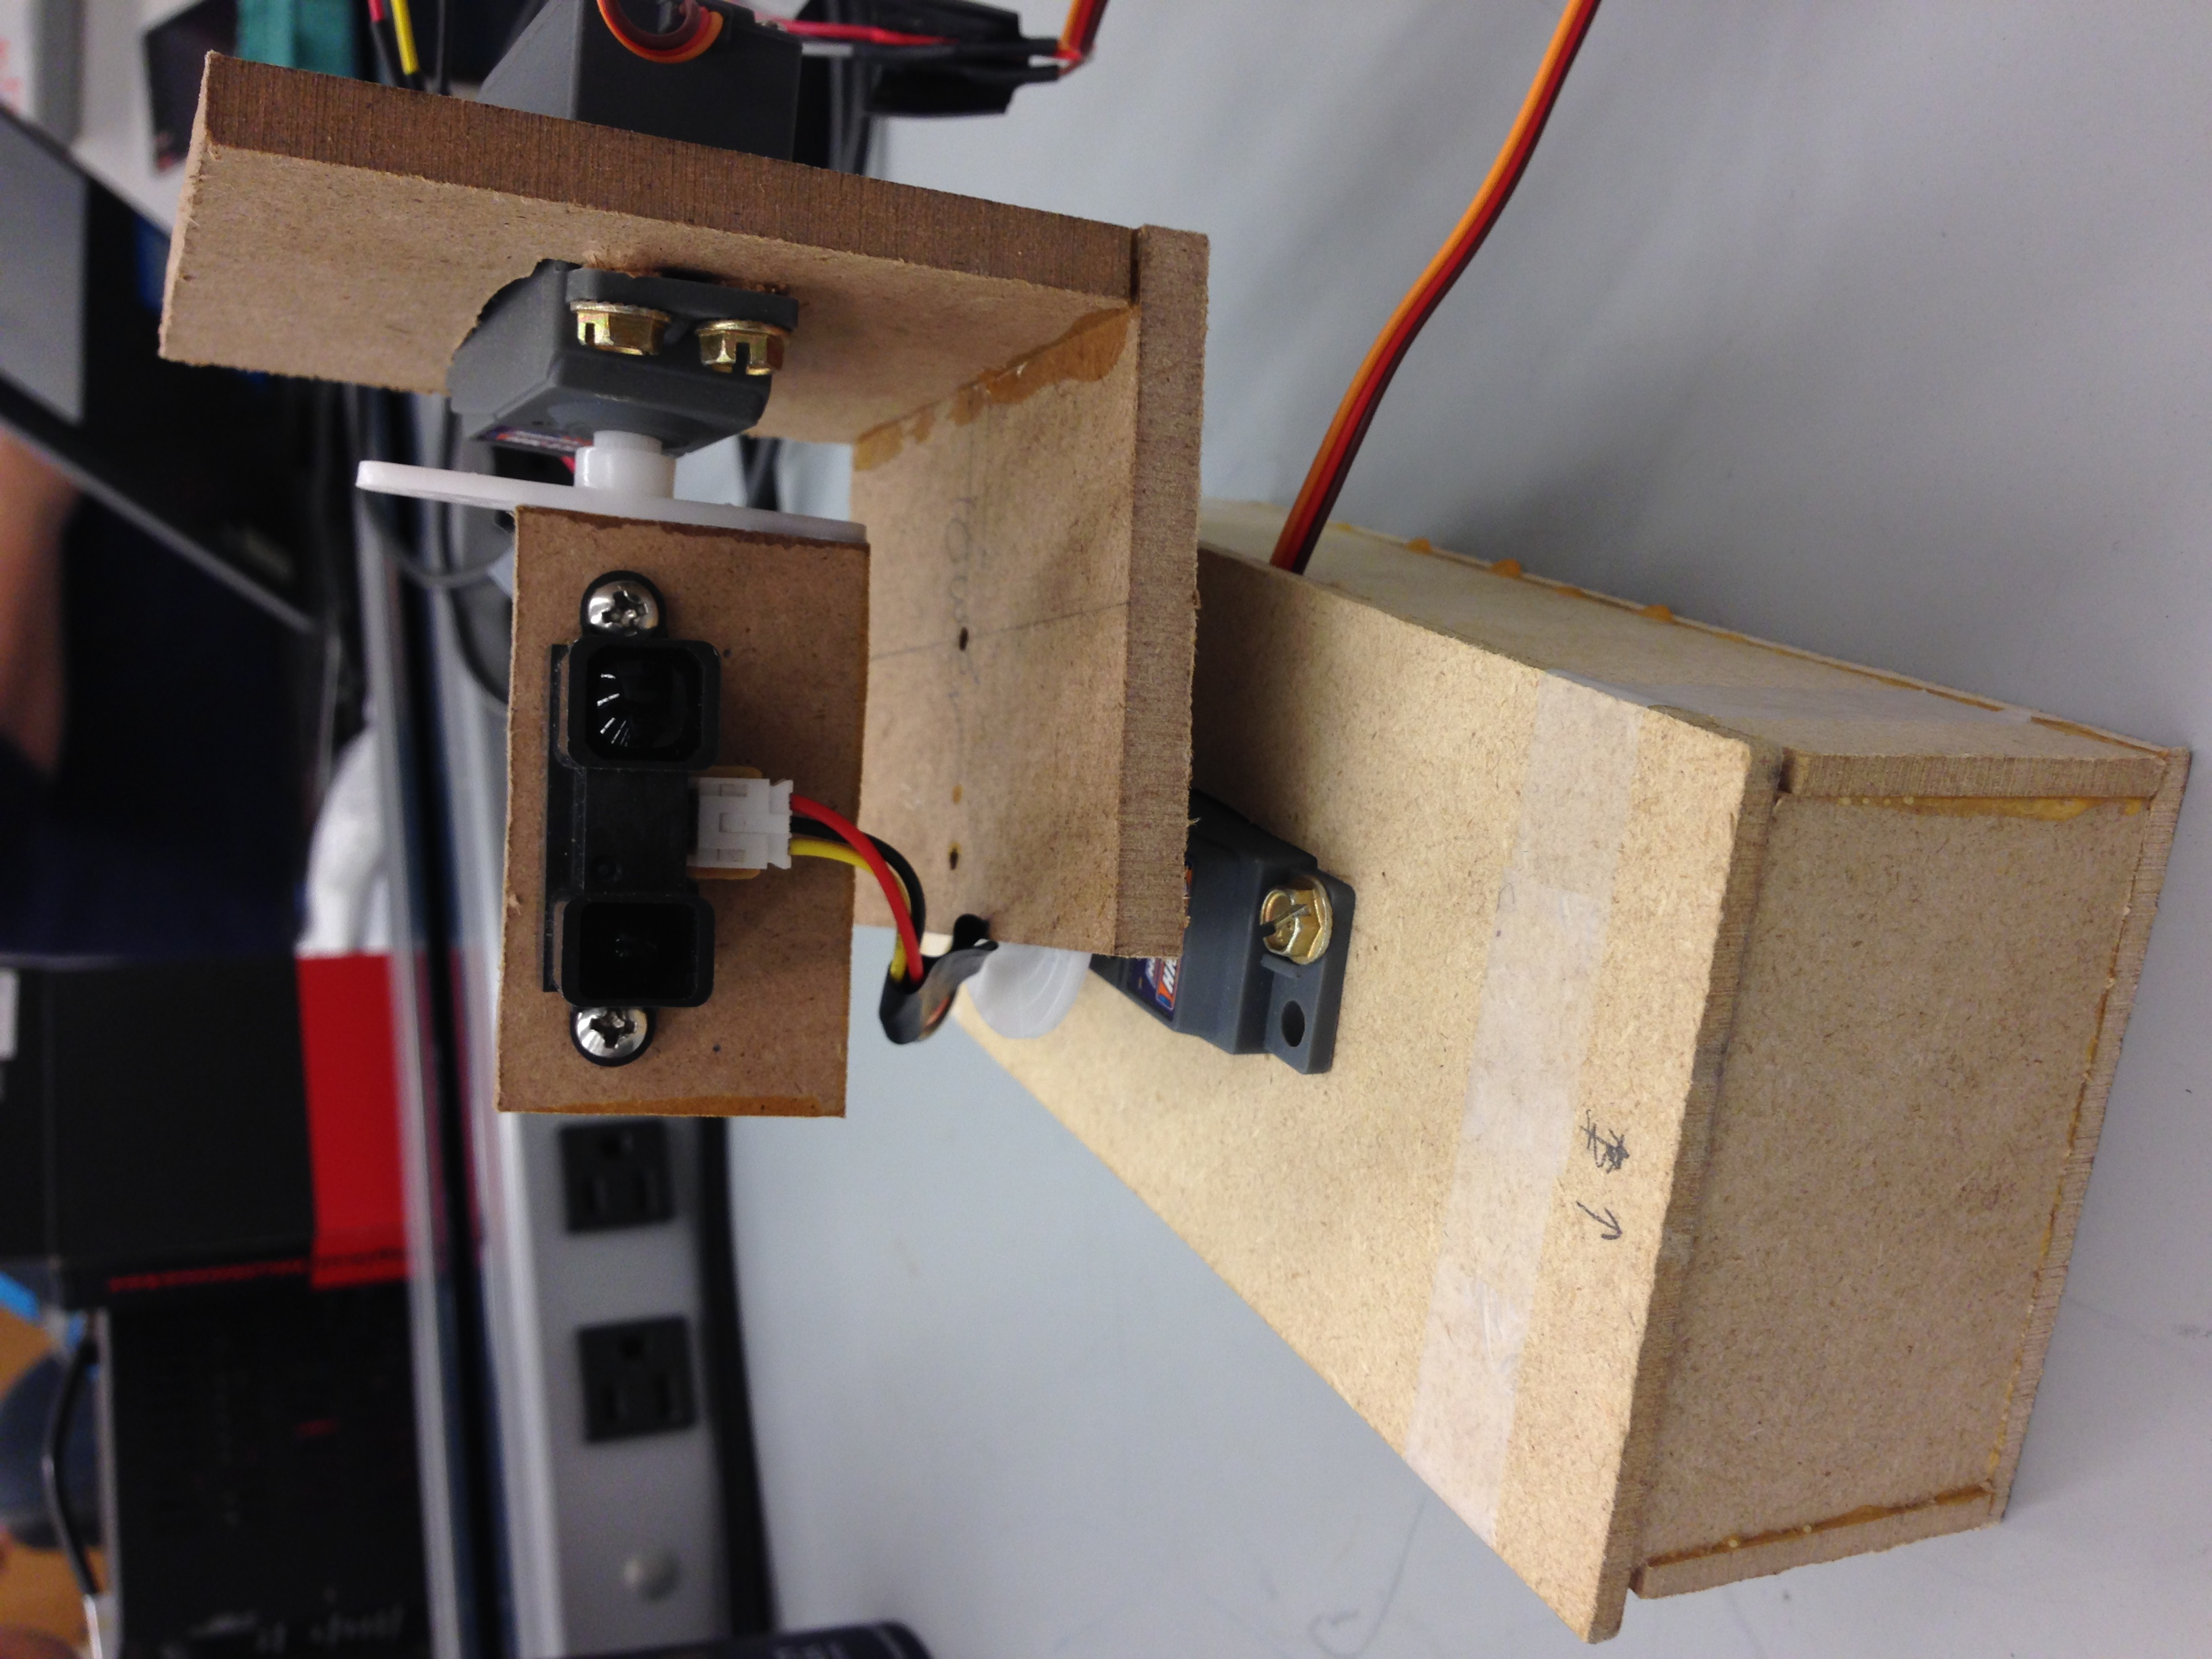
\includegraphics[scale=0.08, angle=270]{mechanism.JPG}
\caption{Picture of Mechanical Design}
\end{center}
\end{figure}
%

\section{Connection Schematic} \ \\
Below is the schematic showing the pins that we connected the two servos and the infrared range finder to:

\begin{figure}[h!]
\begin{center}
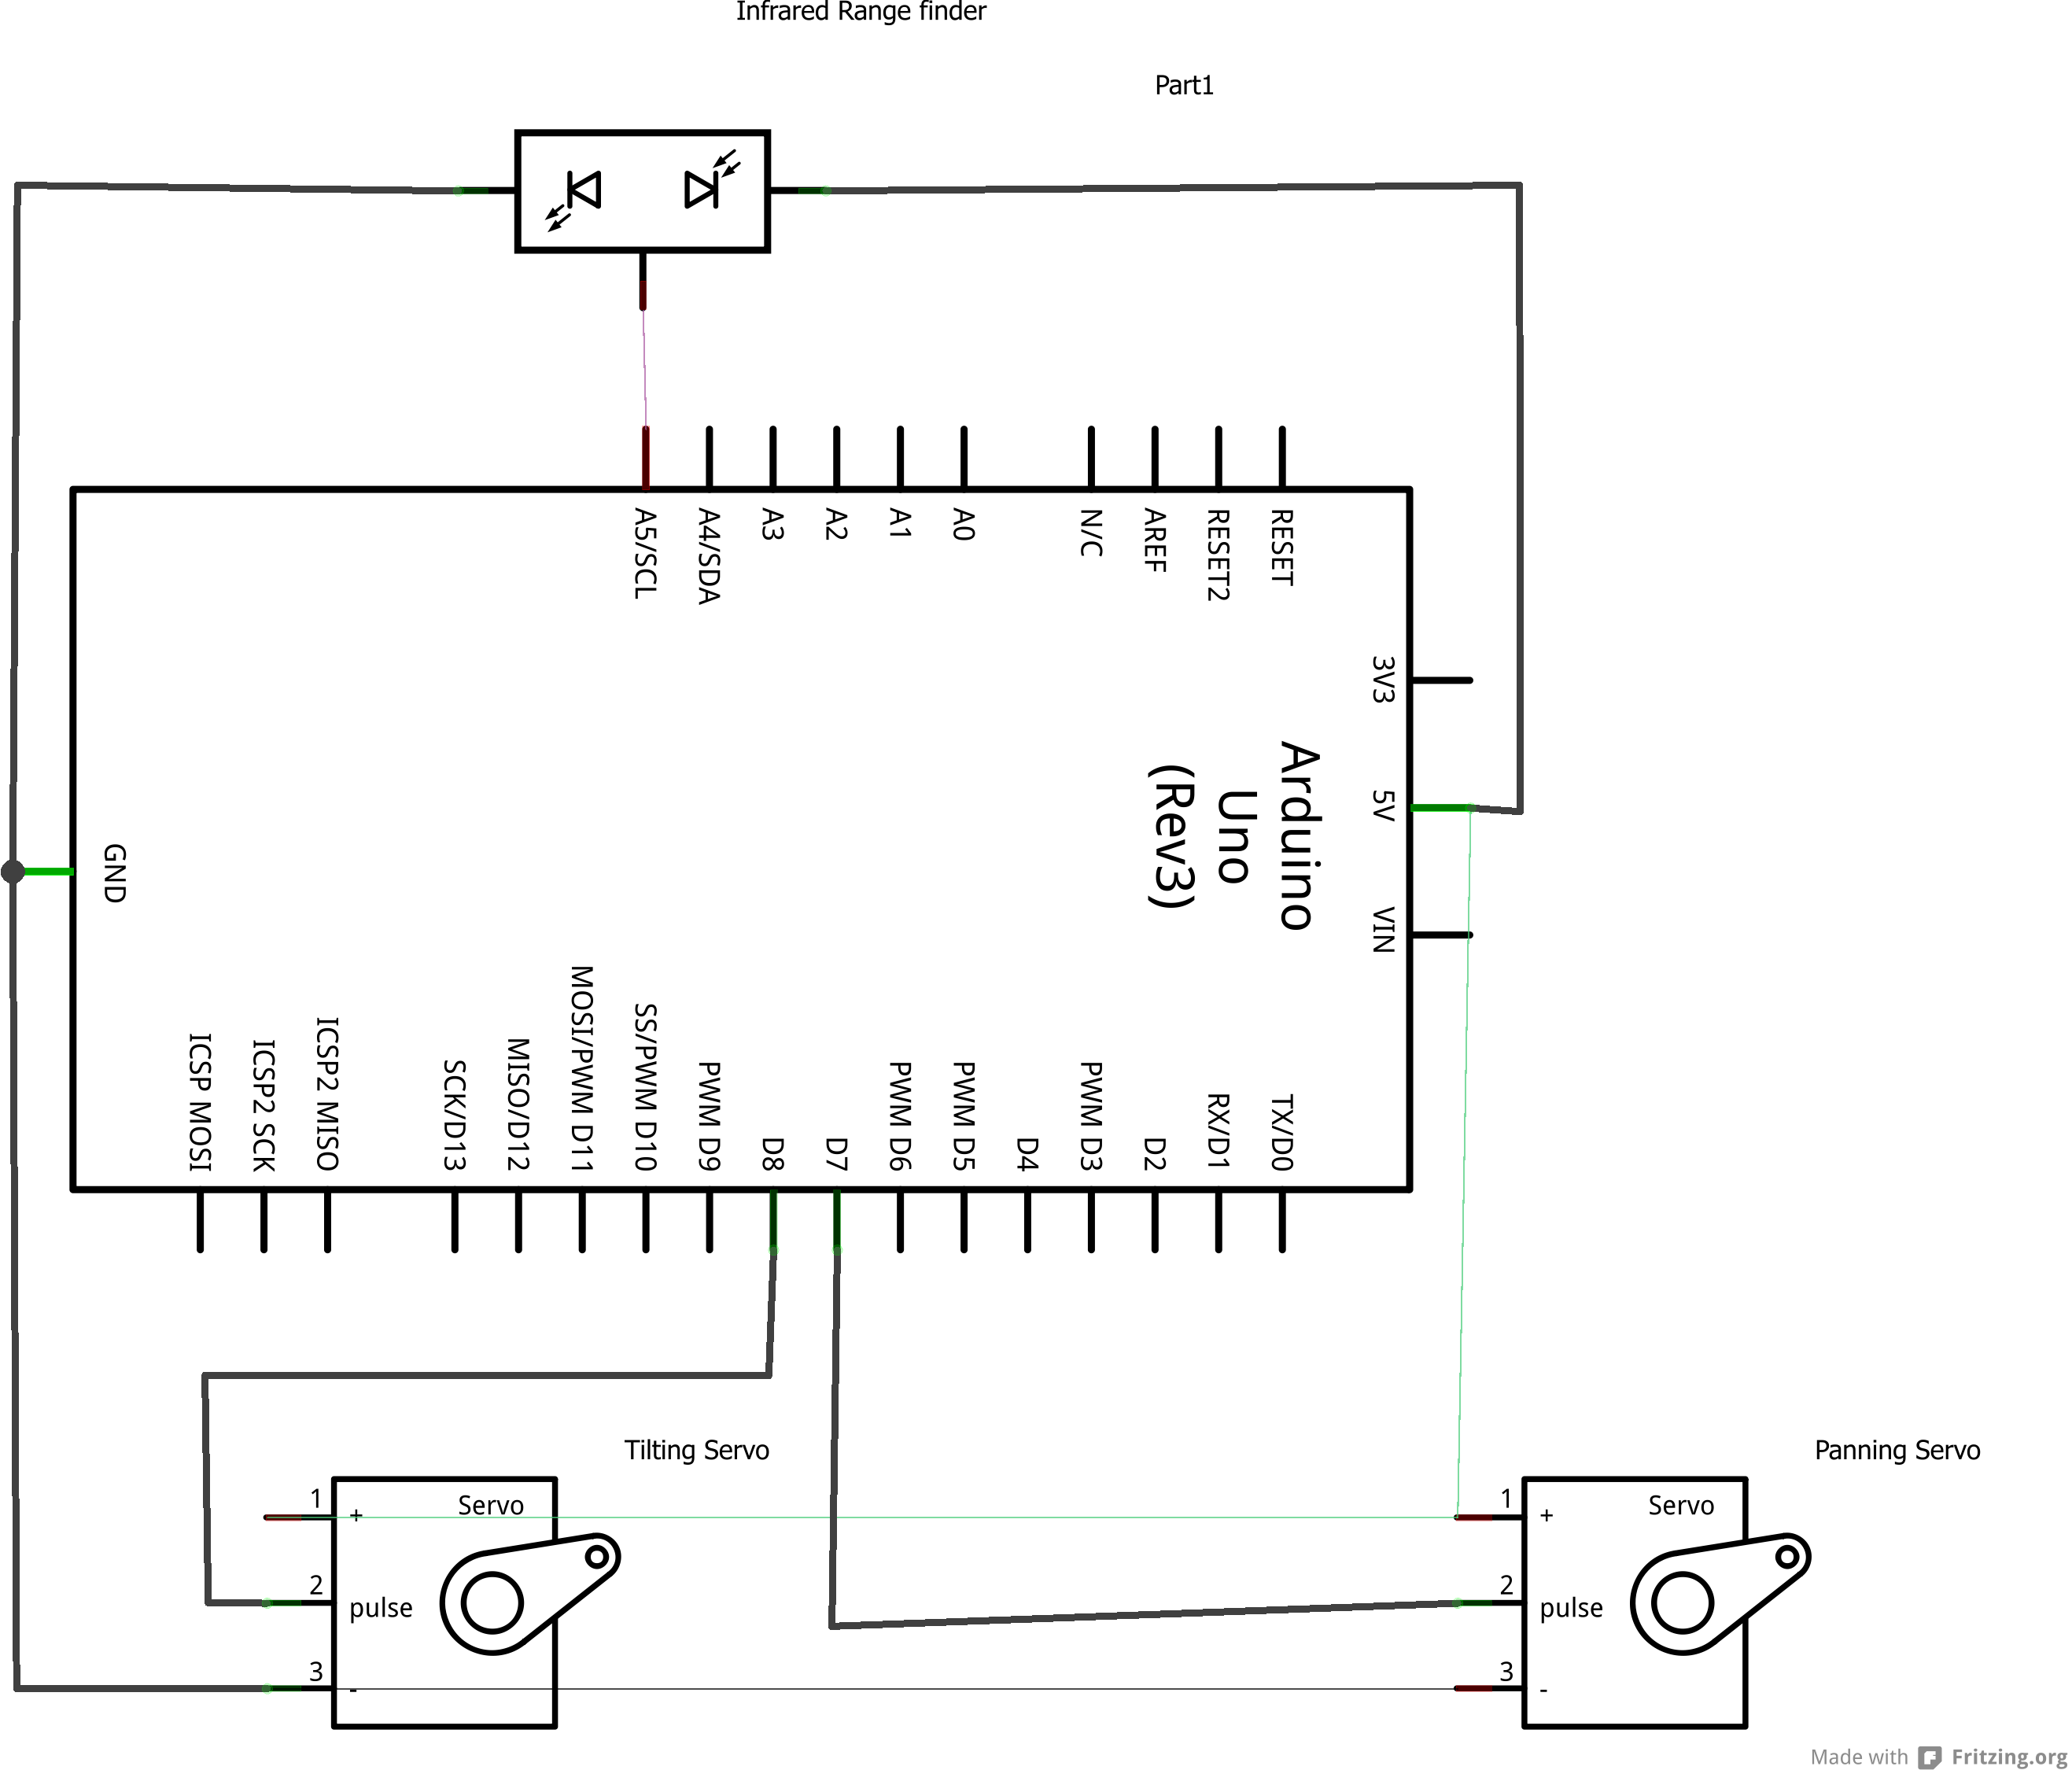
\includegraphics[scale=0.4, angle=270]{schematic.png}
\caption{Schematic of the connections of the servos and infrared range finder}
\end{center}
\end{figure}

\section{Sensor Testing} \ \\
The infrared range finder outputs a voltage that corresponds to the distance it detects. However, according to the data sheet, that relationship is not linear. Hence we had to calibrate our own sensors and figure out that relationship experimentally. \\

In order to do this, we taped a sheet of paper to the wall and placed a tape measure on the ground in order to measure the actual distance our sensor was from the wall. We then proceeded to collect the sensor readings output from the arduino. Although the sensor output is in volts, the arduino converts that to a scale of 0 - 1023 thus the readings we obtain are between 0 and 1023 in value. \\

Once we had obtained sensor readings from the sensor for a distance range of 20cm - 150cm in steps of 10, we then produced a graph of raw sensor reading against distance:


\begin{figure}[h!]
\begin{center}
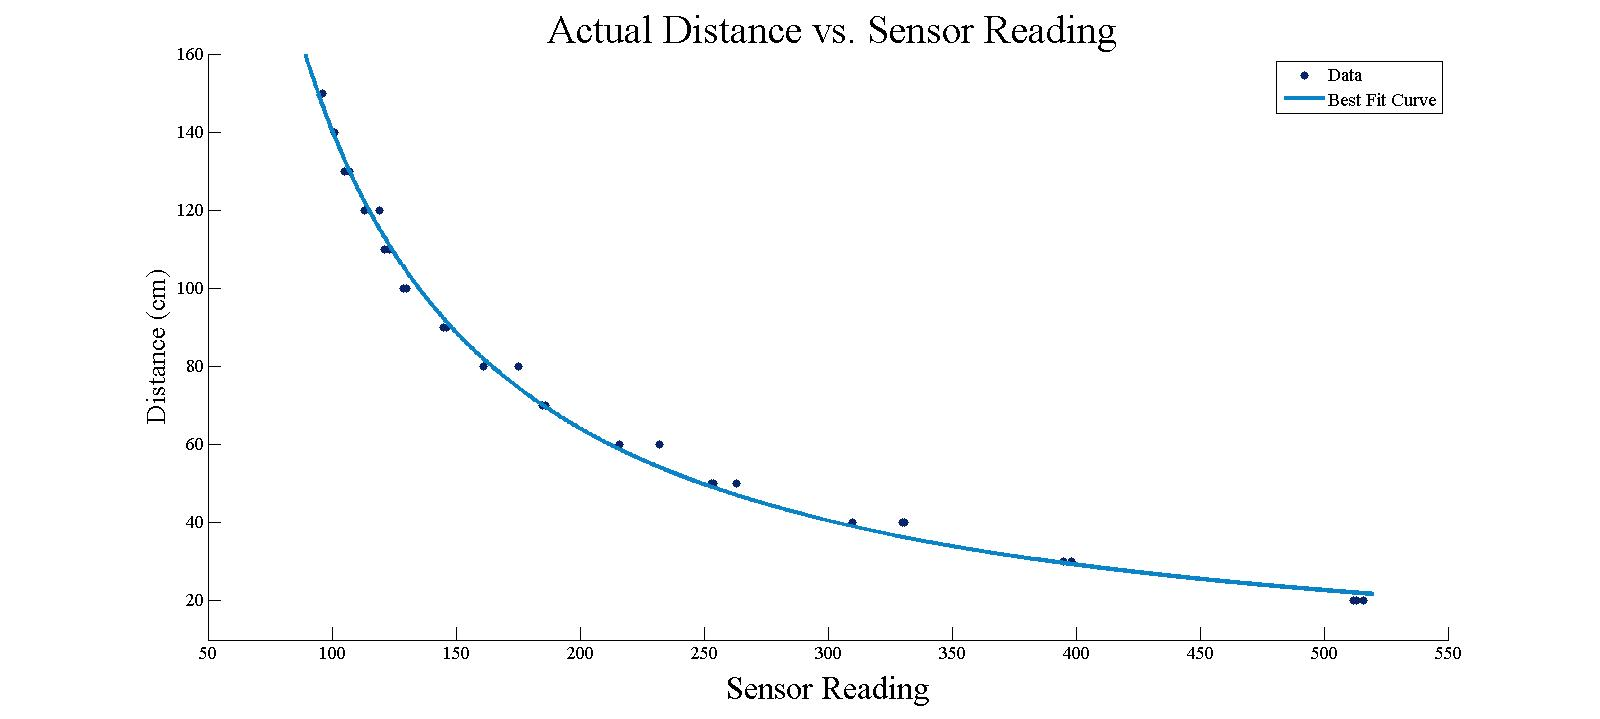
\includegraphics[scale=0.3]{ReadingDistance.jpg}
\caption{Graph of Actual Distance against Sensor Reading with the best fit curve plotted as well}
\end{center}
\end{figure}

As shown in the figure above, we used the curve fitting tool to find the equation of the line that would fit the data. We eventually found out that the equation that related our raw sensor output to distance was:

\begin{equation}
distance=25732.835((sensor reading^{-1.13146})
\end{equation}
%
With this equation now known, we programmed it into the arduino to convert the raw sensor readings into distance. We then repeated the data collection method above but recorded calculated distance data instead of raw sensor data. We then plotted actual distance against distance calculated by the arduino:
%
\begin{figure}[h!]
\begin{center}
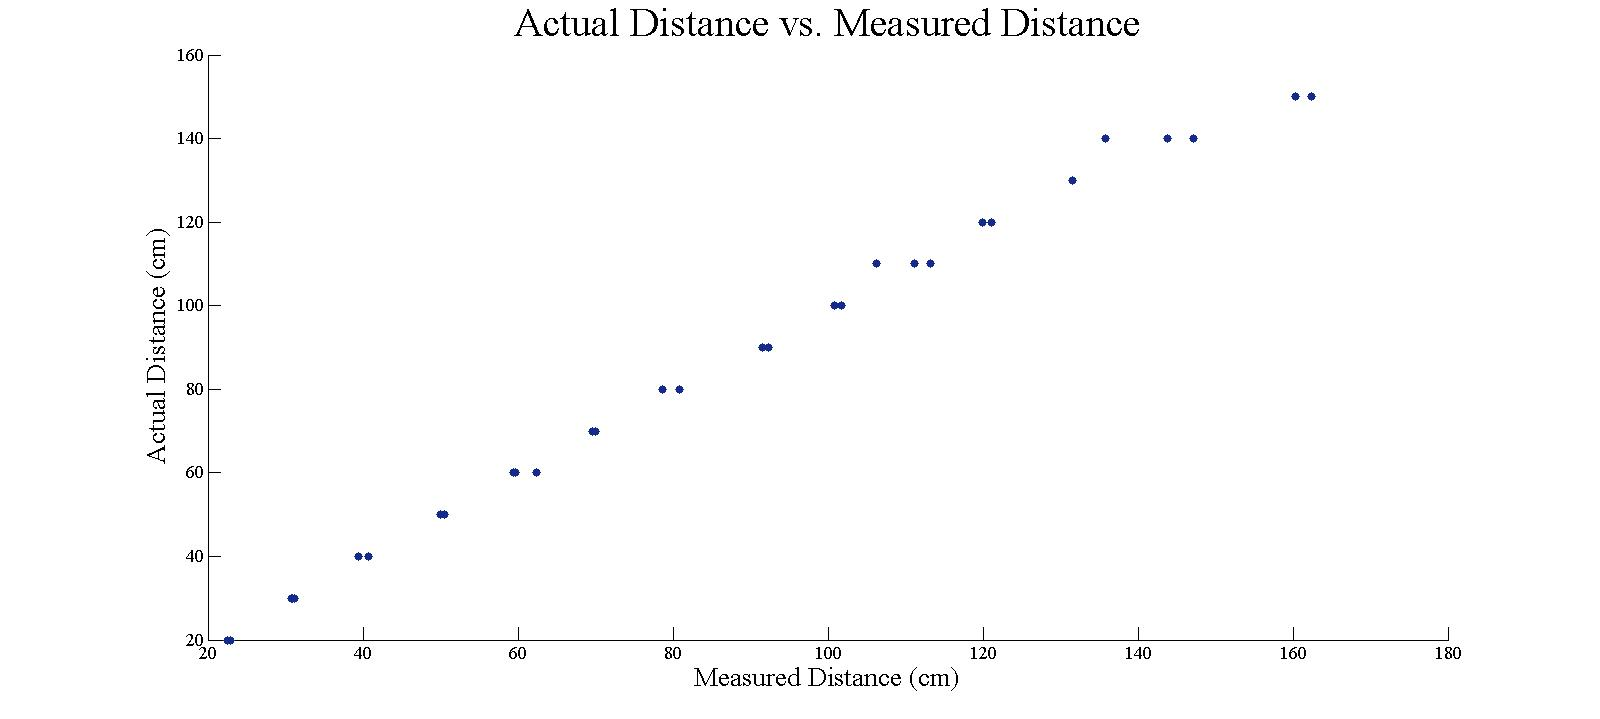
\includegraphics[scale=0.3]{MeasuredActual.jpg}
\caption{Graph of Actual Distance against calculated distance plotted as a scatter plot}
\end{center}
\end{figure}
%
As can be seen in figure 3, the data is approximately linear and the scatter of the data suggests that the sensor readings are pretty accurate. However, the further the actual distance, the larger the scatter and the less accurate the readings.

\section{One Servo Sensor} \ \\
%
In order to avoid building multiple mechanisms for one servo and then two servos, we designed a mechanism for two servos. In order to take a 2D plot, we set the vertical angle to 90 degrees in order to point the sensor straight ahead. We then perform a full sweep of the horizontal angles once through. \\

A picture of the sensor taking a horizontal sweep is shown below: \\

\begin{figure}[h!]
\begin{center}
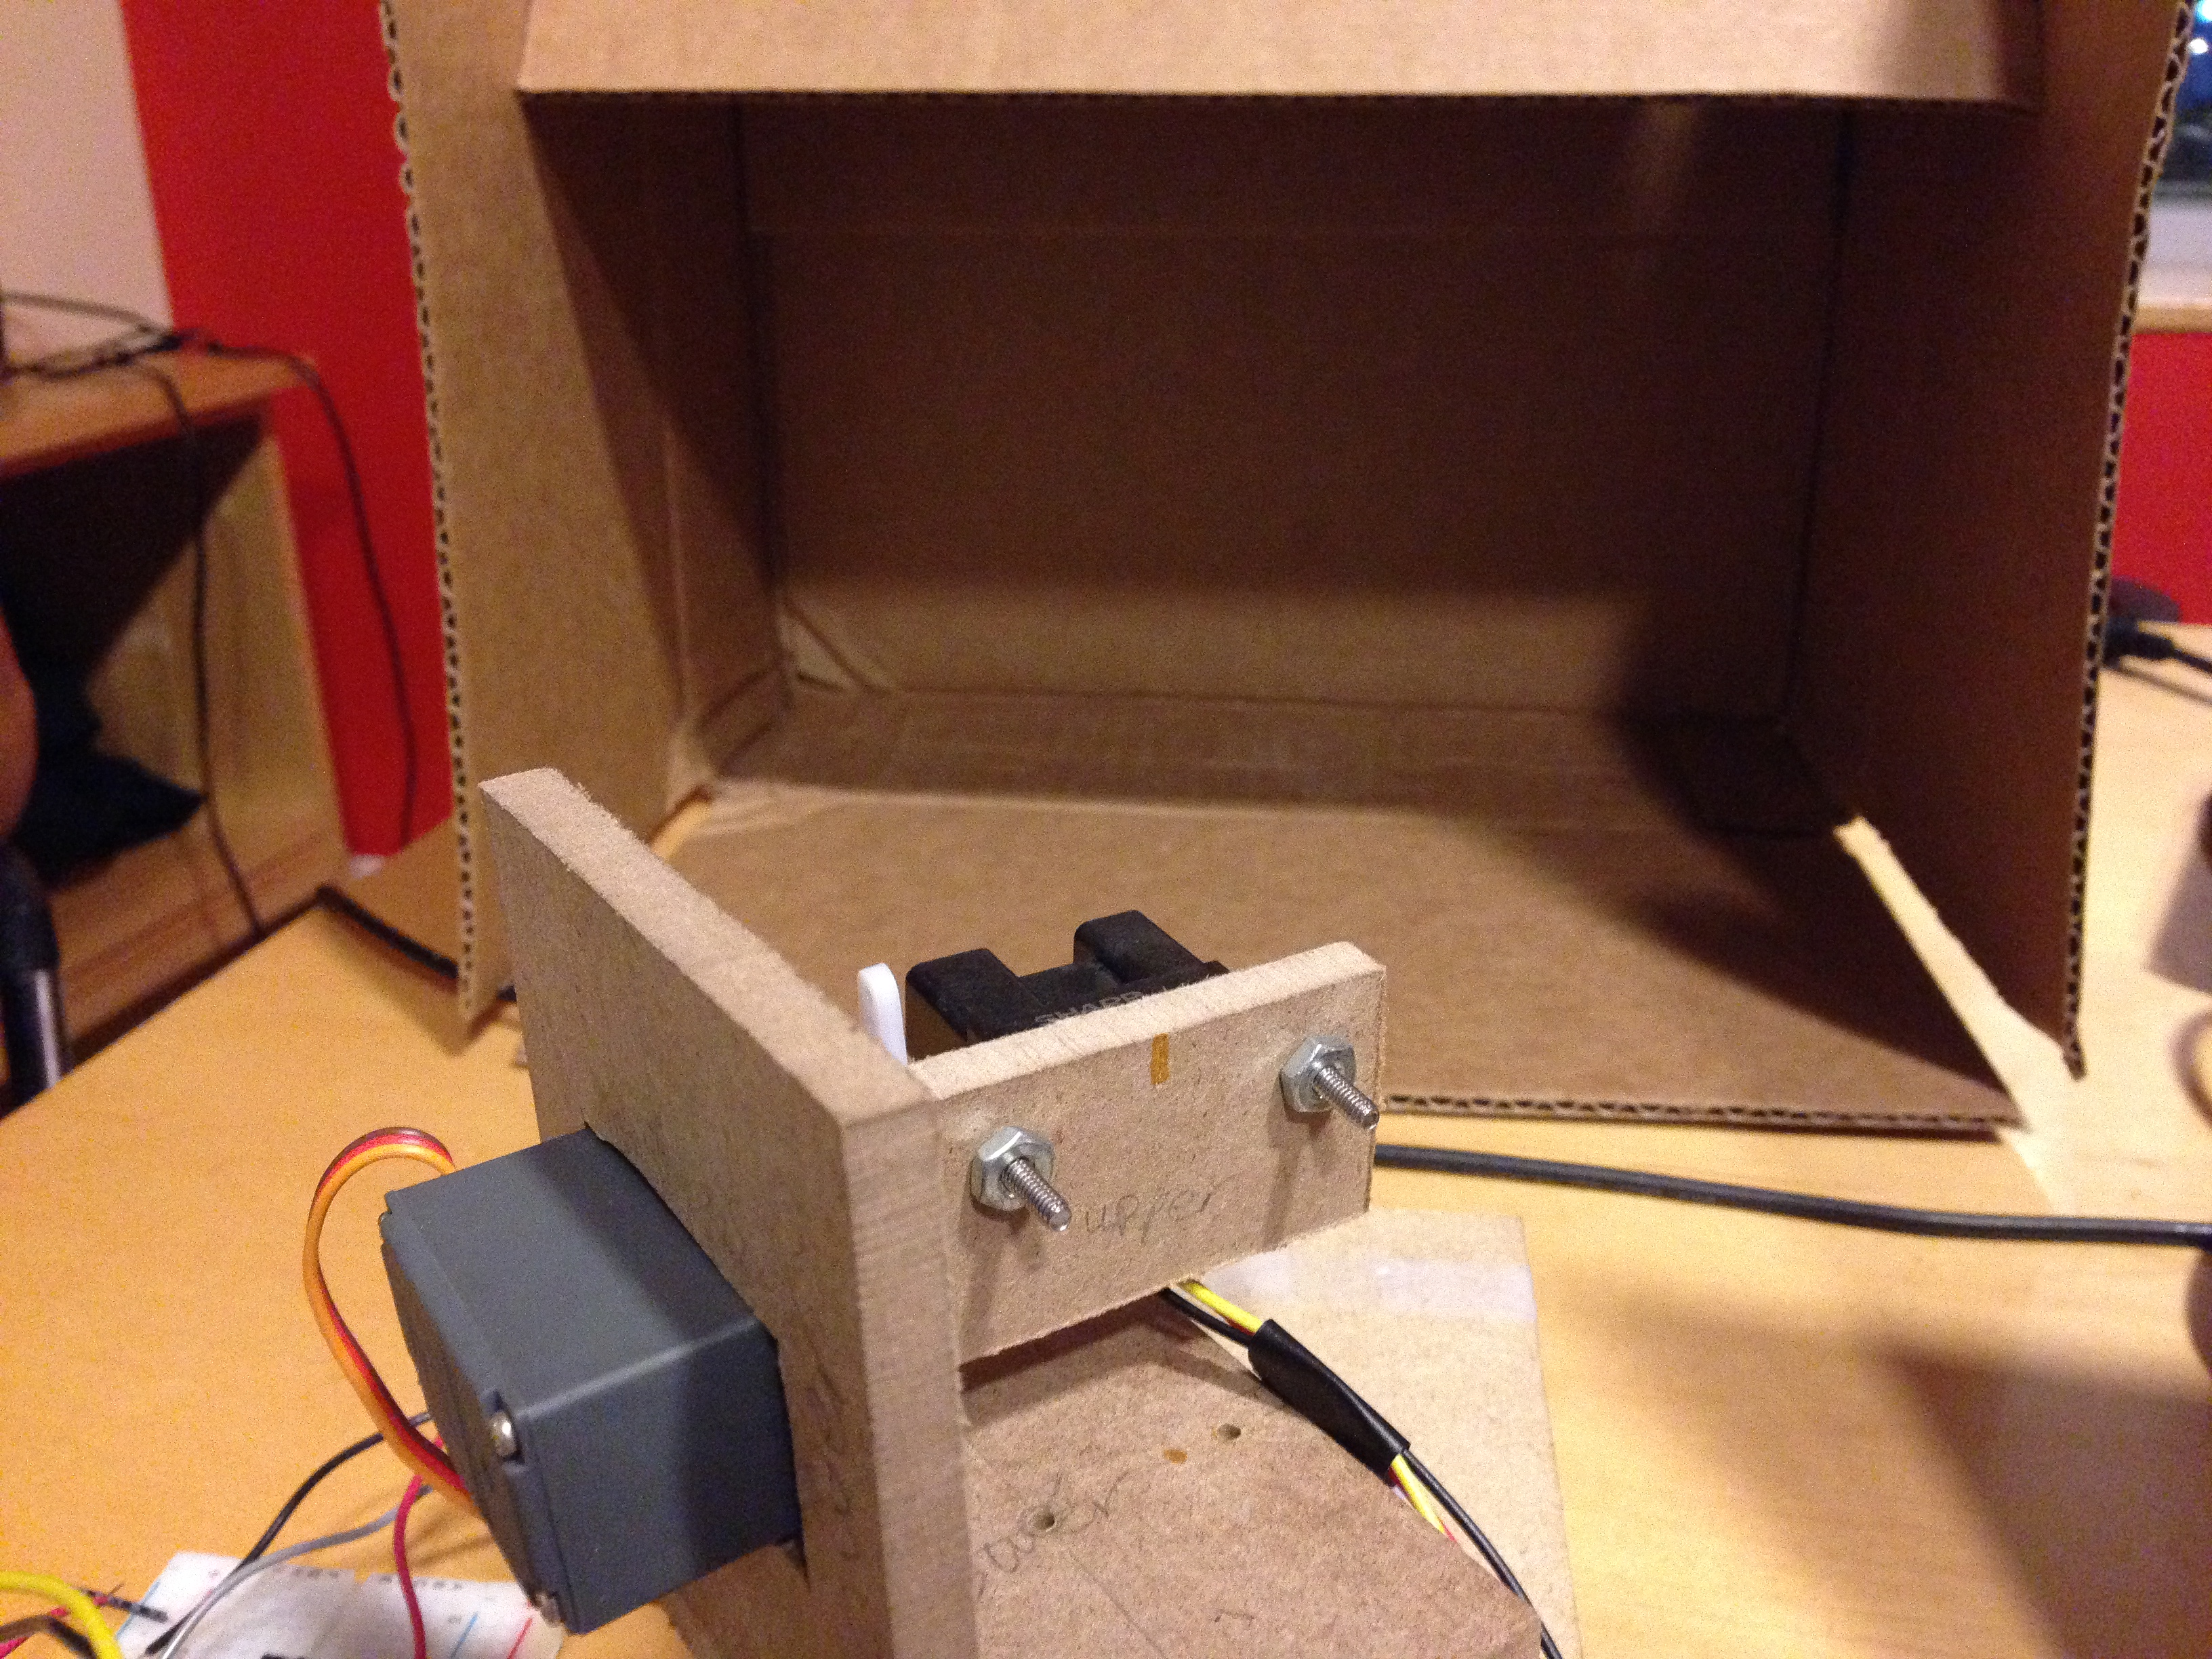
\includegraphics[scale=0.08]{2dscanpic.JPG}
\caption{The sensor taking a 2-D scan of the inside of a cardboard box}
\end{center}
\end{figure}
\newpage

The output of that scan is now shown below:

\begin{figure}[h!]
\begin{center}
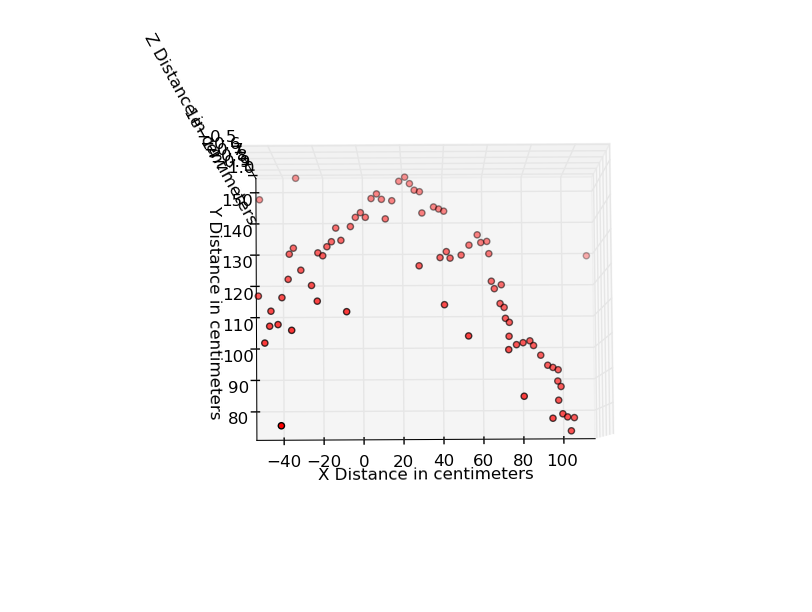
\includegraphics[scale=0.6]{2d_scan.png}
\caption{2-D scan output of the sensor}
\end{center}
\end{figure}

\section{Two Servo Sensor} \ \\
%
For this part, we used the same mechanical set up as before. However, we made it perform both a horizontal and vertical sweep instead of just a horizontal sweep. A picture of the sensor taking a 3D sweep of the diorama is shown below:

\begin{figure}[h!]
\begin{center}
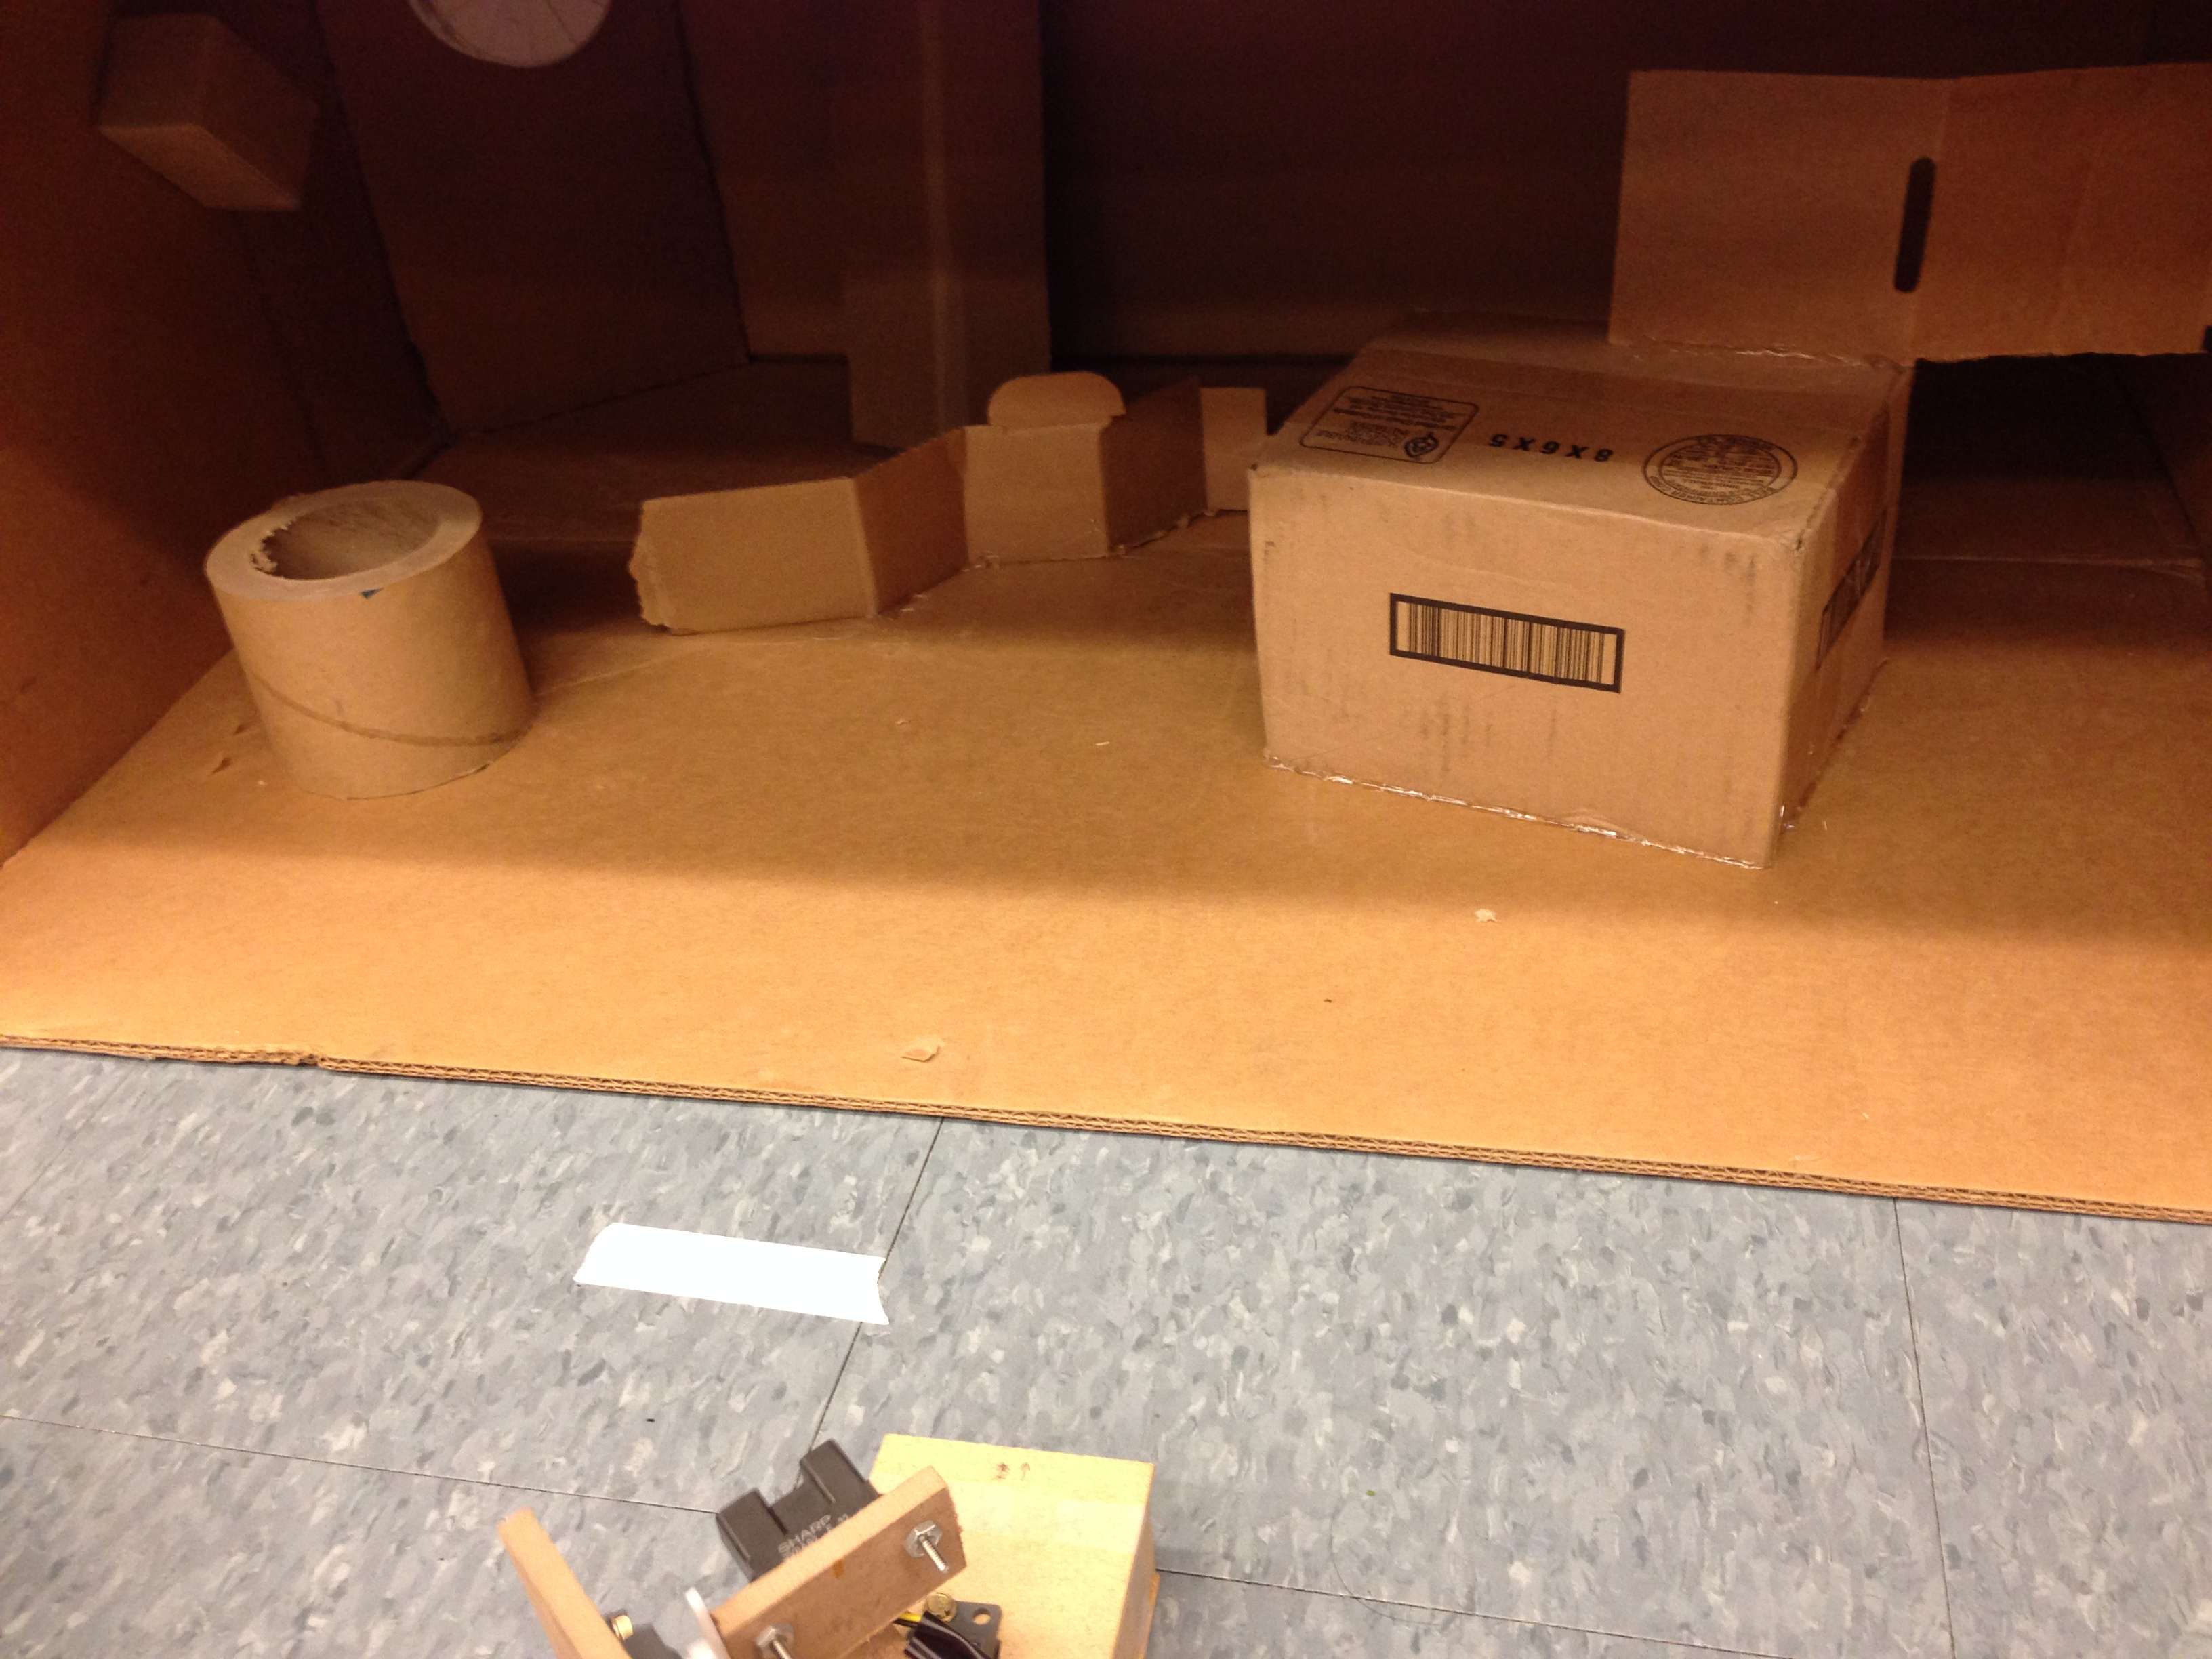
\includegraphics[scale=0.06]{3dscan.JPG}
\caption{The LIDAR taking a 3-D scan of the diorama}
\end{center}
\end{figure}
%
The 3D output of our python programme is shown on the next page:
%
\begin{figure}[h!]
\begin{center}
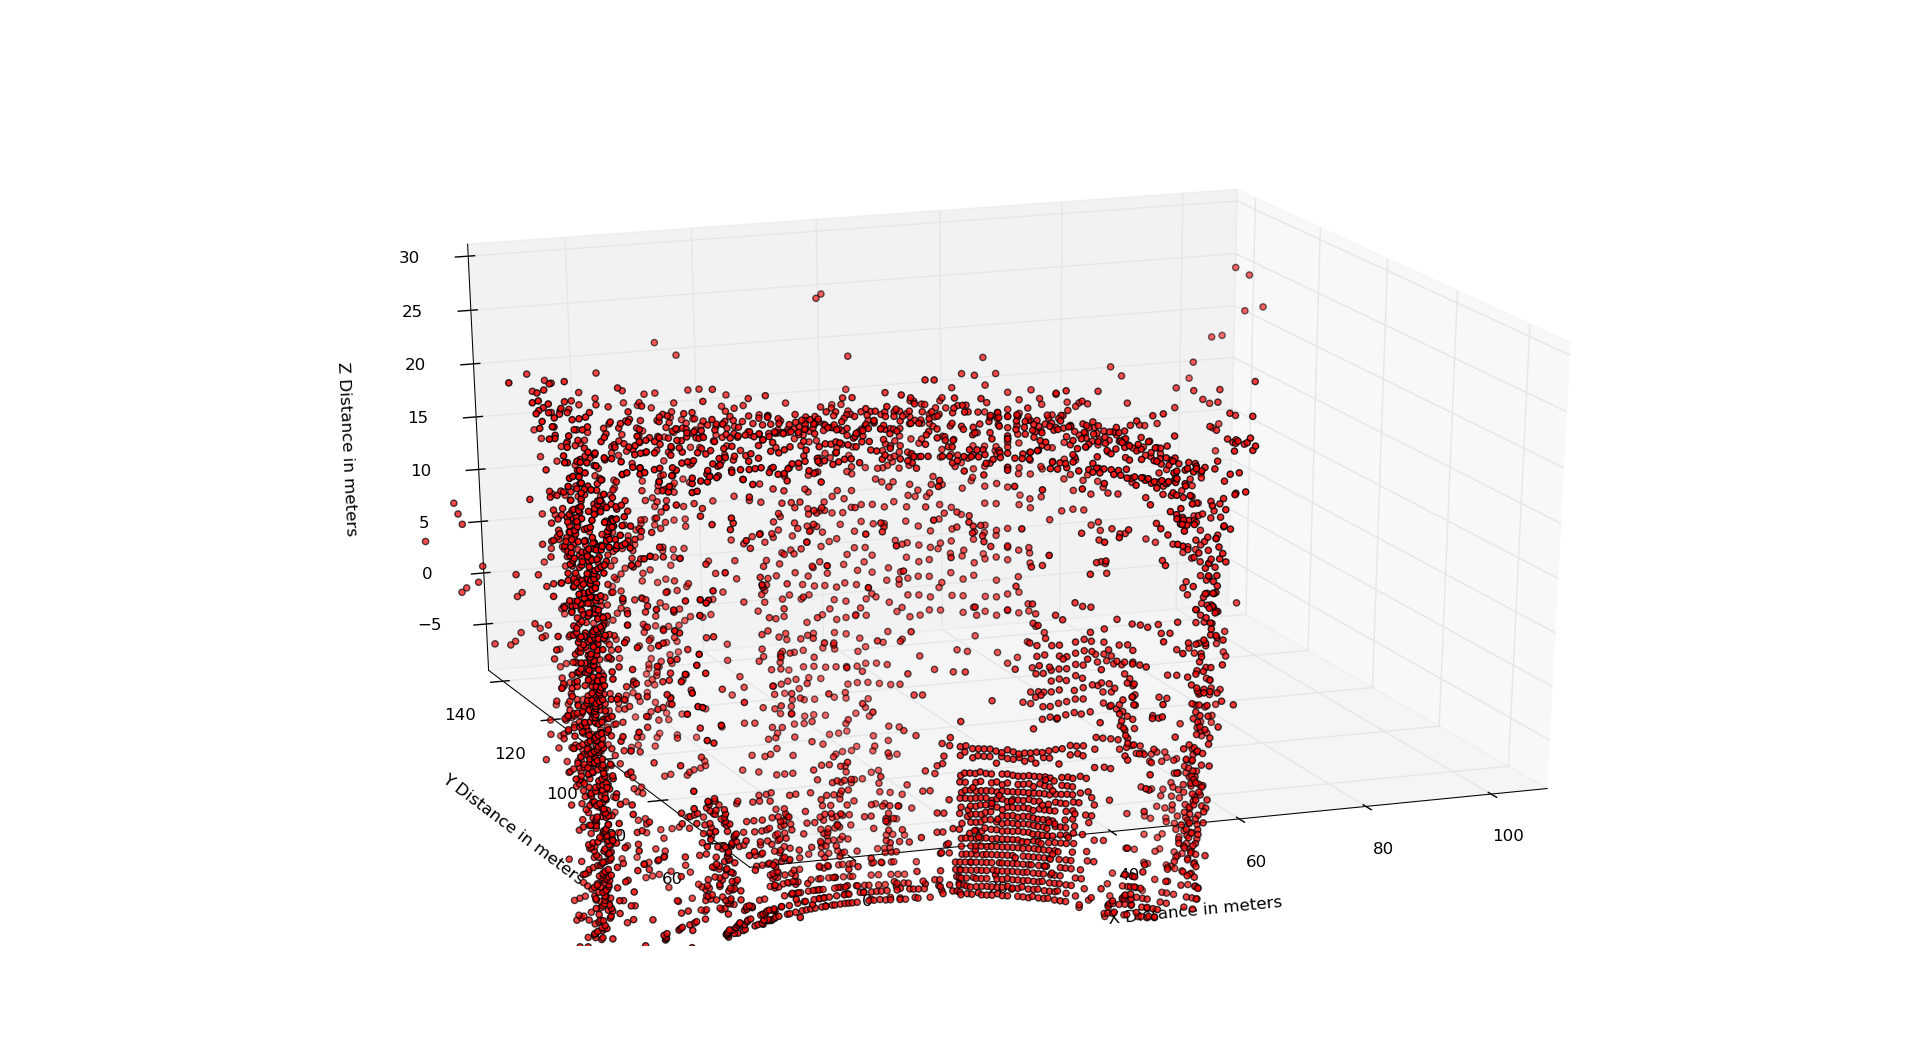
\includegraphics[scale=0.4]{3D_diarama2.png}
\caption{3D plot of the Diorama used for this class; It has been zoomed in for a better view}
\end{center}
\end{figure}

The 3D plot looks similar to the diorama, especially towards the front. Both the box and roll in the front of the diorama are identifiable in the picture. However, the further back in the diorama, the less accurate our representation is, hence the lack of detail toward the back of the diarama. In addition, the bottom right corner of the diorama is not very well depicted. This is because we set our LIDAR up at an angle where the box in the front of the diorama blocks that corner.


\section{Code} \ \\
In essence, our code has two main modules to it: one written in python and one written in arduino code. \\

The arduino code is written to only contain modes of operation. The available modes of operation are as follows:

\begin{enumerate}

\item Mode '1': Move panning servo to the right by 1 degree
\item Mode '2': Move panning servo to the left by 1 degree
\item Mode '3': Move tilting servo up by 1 degree
\item Mode '4': Move tilting servo down by 1 degree
\item Mode '5': Move the panning servo to the home position as defined at the beginning of the code
\item Mode '6': Move the tilting servo to the home position as defined at the beginning of the code
\item Mode '7': Take a reading from the infrared range finder and return the distance measured to the serial port for python to read
\item Mode '8': Put the current vertical and horizontal angle together into a string to output to the serial port for python to read

\end{enumerate}


Hence, the arduino simply waits for a command to be passed to it from python through the serial port. Once it receives a command in the form of a mode number, it executes the code corresponding to the mode number received and carries out the action. \\

The python code is more complex. The python code has full control of the entire operation of scanning the 3D space, collecting the data, performing the trigonometry necessary to convert spherical co-ordinates to cartesian co-ordinates and then finally producing the 3-D plot. \\

The communication between the python code and the arduino is done entirely through the serial port using the python serial module. The act of scanning the space is done by iterating through a range of horizontal and vertical angles, both in increments of 1 degree. The sensor begins at the pre-defined home position. In the case of the diorama used for this lab, the home position is defined as 135 degrees with respect to the horizontal axis and 74 degrees with respect to the vertical. The reference for these angles is shown below: \\

\begin{figure}[h!]
\begin{center}
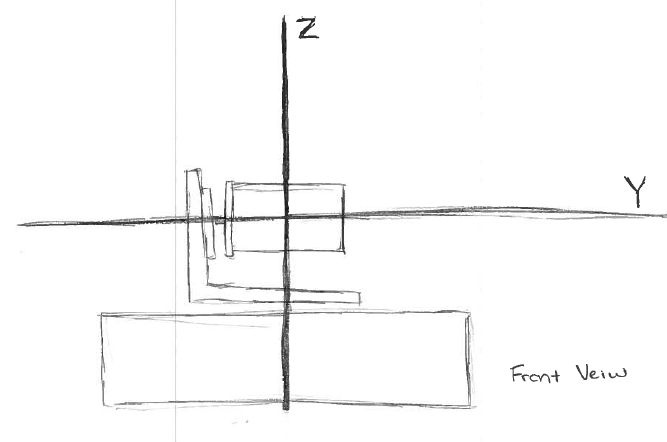
\includegraphics[scale=0.3]{FrontView.PNG}
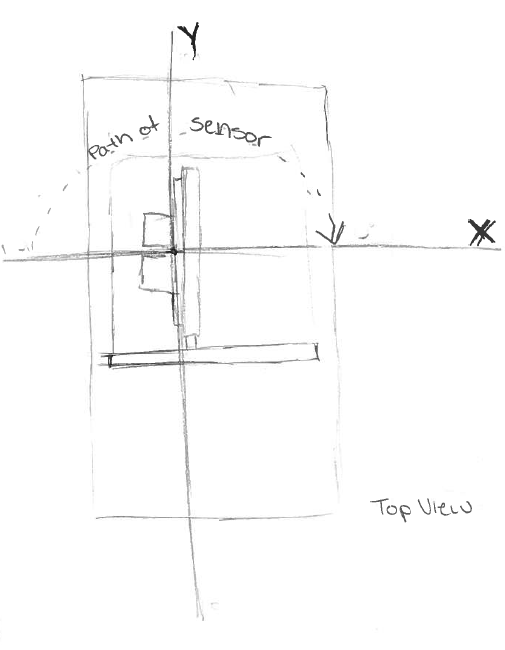
\includegraphics[scale=0.3]{TopView.PNG}
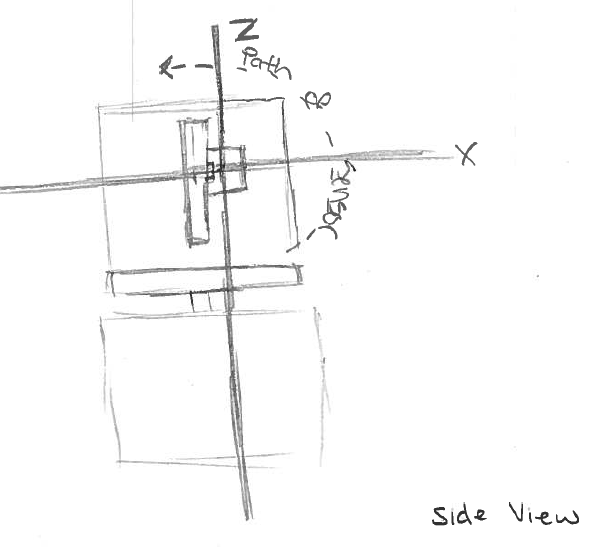
\includegraphics[scale=0.3]{SideView.PNG}
\caption{Diagrams showing the reference used to determine the angle of the sensor when converting from spherical to cartesian co-ordinates}
\end{center}
\end{figure}

From the home position, for each horizontal angle, the python code performs the following steps:

\begin{enumerate}
\item Instructs the arduino to take a reading and return the distance measured by the sensor through the serial port
\item Instructs the arduino to read the current vertical and horizontal angle and concatenate it into one string. Then return it through the serial port for python to read
\item Feed the distance reading and the vertical and horizontal angles to a new lidar object as defined in python (see appendix for the full class definition). The initialized lidar object will then take those numbers and convert them from spherical co-ordinates to cartesian co-ordinates. It then stores the cartesian co-ordinates as instance variables.
\item Appends the newly created lidar object to the data list to retrieve later for plotting.
\item Move the sensor 1 degree to the right
\end{enumerate}

Once the arduino has completed a full horizontal sweep at a given tilt angle, it then resets back to the horizontal home position and increases the vertical angle by 1 degree. It then proceeds to sweep through the horizontal angles again as described in the above list. \\

Once the full 3D sweep of the space is complete, the python code then reads each lidar object in the data list and produces a 3D scatter plot of the data obtained from the scan as a matplotlib figure.

\end{document}